\section{Spark::Sp\-Matrix$<$ N, Real $>$ Class Template Reference}
\label{classSpark_1_1SpMatrix}\index{Spark::SpMatrix@{Spark::SpMatrix}}
{\tt \#include $<$Sp\-Matrix.h$>$}

Inheritance diagram for Spark::Sp\-Matrix$<$ N, Real $>$:\begin{figure}[H]
\begin{center}
\leavevmode
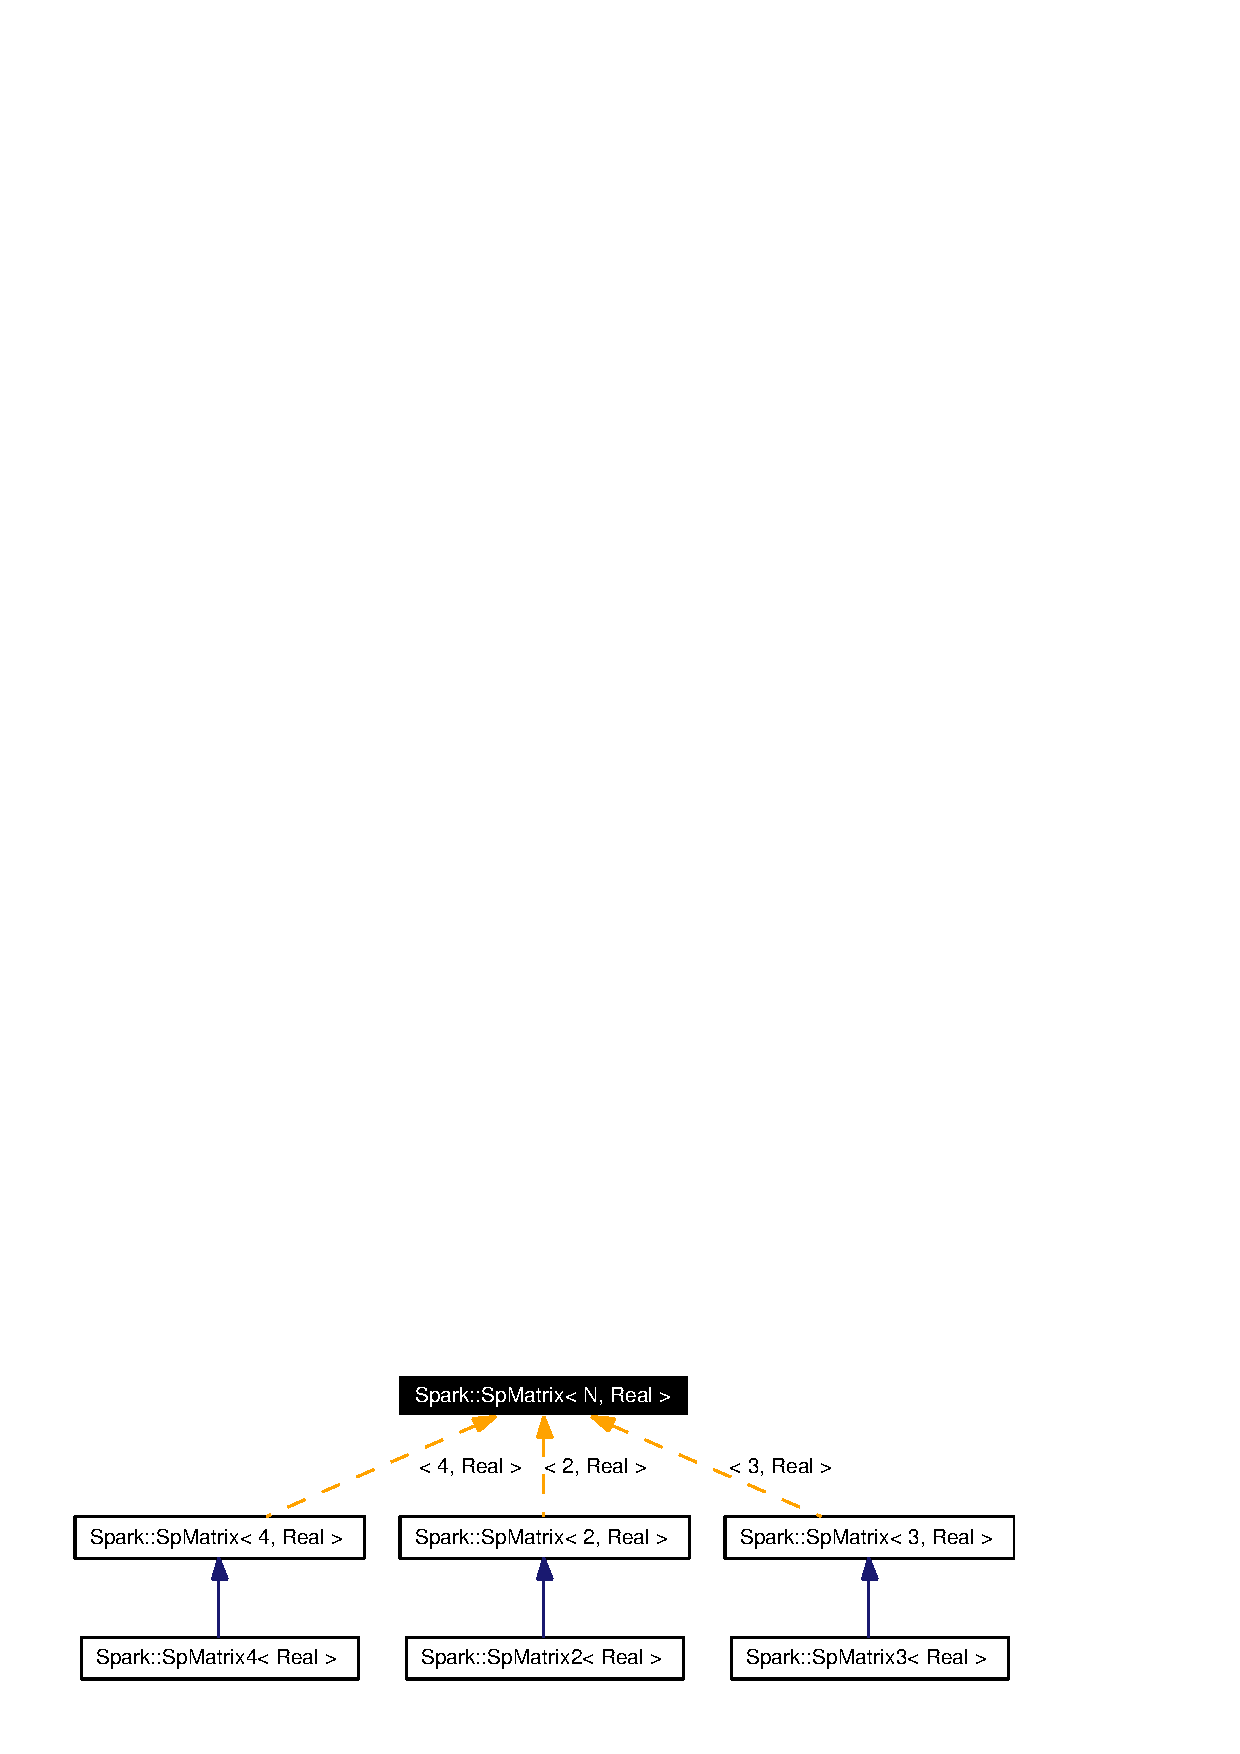
\includegraphics[width=243pt]{classSpark_1_1SpMatrix__inherit__graph}
\end{center}
\end{figure}
Collaboration diagram for Spark::Sp\-Matrix$<$ N, Real $>$:\begin{figure}[H]
\begin{center}
\leavevmode
\includegraphics[width=88pt]{classSpark_1_1SpMatrix__coll__graph}
\end{center}
\end{figure}


\subsection{Detailed Description}
\subsubsection*{template$<$unsigned int N, class Real$>$ class Spark::Sp\-Matrix$<$ N, Real $>$}

Nx\-N Matrix base class for vector algebra. 

Definition at line 34 of file Sp\-Matrix.h.\subsection*{Public Member Functions}
\begin{CompactItemize}
\item 
{\bf Sp\-Matrix} ()
\item 
{\bf Sp\-Matrix} (bool b\-Zero)
\item 
{\bf Sp\-Matrix} (const {\bf Sp\-Matrix} \&rk\-M)
\item 
{\bf operator const Real $\ast$} () const
\item 
{\bf operator Real $\ast$} ()
\item 
const Real $\ast$ {\bf operator[$\,$]} (unsigned int ui\-Row) const
\item 
Real $\ast$ {\bf operator[$\,$]} (unsigned int ui\-Row)
\item 
Real {\bf operator()} (unsigned int ui\-Row, unsigned int ui\-Col) const
\item 
Real \& {\bf operator()} (unsigned int ui\-Row, unsigned int ui\-Col)
\item 
{\bf Sp\-Tuple}$<$ N, Real $>$ {\bf get\-Row} (unsigned int ui\-Row) const
\item 
void {\bf set\-Row} (unsigned int ui\-Row, const {\bf Sp\-Tuple}$<$ N, Real $>$ \&rk\-V)
\item 
{\bf Sp\-Tuple}$<$ N, Real $>$ {\bf get\-Column} (unsigned int ui\-Col) const
\item 
void {\bf set\-Column} (unsigned int ui\-Col, const {\bf Sp\-Tuple}$<$ N, Real $>$ \&rk\-V)
\item 
{\bf Sp\-Matrix} \& {\bf operator=} (const {\bf Sp\-Matrix} \&rk\-M)
\item 
bool {\bf operator==} (const {\bf Sp\-Matrix} \&rk\-M) const
\item 
bool {\bf operator!=} (const {\bf Sp\-Matrix} \&rk\-M) const
\item 
bool {\bf operator$<$} (const {\bf Sp\-Matrix} \&rk\-M) const
\item 
bool {\bf operator$<$=} (const {\bf Sp\-Matrix} \&rk\-M) const
\item 
bool {\bf operator$>$} (const {\bf Sp\-Matrix} \&rk\-M) const
\item 
bool {\bf operator$>$=} (const {\bf Sp\-Matrix} \&rk\-M) const
\item 
{\bf Sp\-Matrix} {\bf operator+} (const {\bf Sp\-Matrix} \&rk\-M) const
\item 
{\bf Sp\-Matrix} {\bf operator-} (const {\bf Sp\-Matrix} \&rk\-M) const
\item 
{\bf Sp\-Matrix} {\bf operator $\ast$} (const {\bf Sp\-Matrix} \&rk\-M) const
\item 
{\bf Sp\-Matrix} {\bf operator $\ast$} (Real f\-Scalar) const
\item 
{\bf Sp\-Matrix} {\bf operator/} (Real f\-Scalar) const
\item 
{\bf Sp\-Matrix} {\bf operator-} () const
\item 
{\bf Sp\-Matrix} \& {\bf operator+=} (const {\bf Sp\-Matrix} \&rk\-M)
\item 
{\bf Sp\-Matrix} \& {\bf operator-=} (const {\bf Sp\-Matrix} \&rk\-M)
\item 
{\bf Sp\-Matrix} \& {\bf operator $\ast$=} (Real f\-Scalar)
\item 
{\bf Sp\-Matrix} \& {\bf operator/=} (Real f\-Scalar)
\item 
{\bf Sp\-Tuple}$<$ N, Real $>$ {\bf operator $\ast$} (const {\bf Sp\-Tuple}$<$ N, Real $>$ \&rk\-V) const
\end{CompactItemize}
\subsection*{Protected Member Functions}
\begin{CompactItemize}
\item 
int {\bf compare} (const {\bf Sp\-Matrix} \&rk\-M) const
\end{CompactItemize}
\subsection*{Protected Attributes}
\begin{CompactItemize}
\item 
Real {\bf m\_\-af\-Values} [N][N]
\end{CompactItemize}


\subsection{Constructor \& Destructor Documentation}
\index{Spark::SpMatrix@{Spark::Sp\-Matrix}!SpMatrix@{SpMatrix}}
\index{SpMatrix@{SpMatrix}!Spark::SpMatrix@{Spark::Sp\-Matrix}}
\subsubsection{\setlength{\rightskip}{0pt plus 5cm}template$<$unsigned int N, class Real$>$ {\bf Spark::Sp\-Matrix}$<$ N, Real $>$::{\bf Sp\-Matrix} ()}\label{classSpark_1_1SpMatrix_a0}


\index{Spark::SpMatrix@{Spark::Sp\-Matrix}!SpMatrix@{SpMatrix}}
\index{SpMatrix@{SpMatrix}!Spark::SpMatrix@{Spark::Sp\-Matrix}}
\subsubsection{\setlength{\rightskip}{0pt plus 5cm}template$<$unsigned int N, class Real$>$ {\bf Spark::Sp\-Matrix}$<$ N, Real $>$::{\bf Sp\-Matrix} (bool {\em b\-Zero})}\label{classSpark_1_1SpMatrix_a1}


\index{Spark::SpMatrix@{Spark::Sp\-Matrix}!SpMatrix@{SpMatrix}}
\index{SpMatrix@{SpMatrix}!Spark::SpMatrix@{Spark::Sp\-Matrix}}
\subsubsection{\setlength{\rightskip}{0pt plus 5cm}template$<$unsigned int N, class Real$>$ {\bf Spark::Sp\-Matrix}$<$ N, Real $>$::{\bf Sp\-Matrix} (const {\bf Sp\-Matrix}$<$ N, Real $>$ \& {\em rk\-M})}\label{classSpark_1_1SpMatrix_a2}




\subsection{Member Function Documentation}
\index{Spark::SpMatrix@{Spark::Sp\-Matrix}!compare@{compare}}
\index{compare@{compare}!Spark::SpMatrix@{Spark::Sp\-Matrix}}
\subsubsection{\setlength{\rightskip}{0pt plus 5cm}template$<$unsigned int N, class Real$>$ int {\bf Spark::Sp\-Matrix}$<$ N, Real $>$::compare (const {\bf Sp\-Matrix}$<$ N, Real $>$ \& {\em rk\-M}) const\hspace{0.3cm}{\tt  [protected]}}\label{classSpark_1_1SpMatrix_b0}


\index{Spark::SpMatrix@{Spark::Sp\-Matrix}!getColumn@{getColumn}}
\index{getColumn@{getColumn}!Spark::SpMatrix@{Spark::Sp\-Matrix}}
\subsubsection{\setlength{\rightskip}{0pt plus 5cm}template$<$unsigned int N, class Real$>$ {\bf Sp\-Tuple}$<$N,Real$>$ {\bf Spark::Sp\-Matrix}$<$ N, Real $>$::get\-Column (unsigned int {\em ui\-Col}) const}\label{classSpark_1_1SpMatrix_a11}


\index{Spark::SpMatrix@{Spark::Sp\-Matrix}!getRow@{getRow}}
\index{getRow@{getRow}!Spark::SpMatrix@{Spark::Sp\-Matrix}}
\subsubsection{\setlength{\rightskip}{0pt plus 5cm}template$<$unsigned int N, class Real$>$ {\bf Sp\-Tuple}$<$N,Real$>$ {\bf Spark::Sp\-Matrix}$<$ N, Real $>$::get\-Row (unsigned int {\em ui\-Row}) const}\label{classSpark_1_1SpMatrix_a9}


\index{Spark::SpMatrix@{Spark::Sp\-Matrix}!operator *@{operator $\ast$}}
\index{operator *@{operator $\ast$}!Spark::SpMatrix@{Spark::Sp\-Matrix}}
\subsubsection{\setlength{\rightskip}{0pt plus 5cm}template$<$unsigned int N, class Real$>$ {\bf Sp\-Tuple}$<$N,Real$>$ {\bf Spark::Sp\-Matrix}$<$ N, Real $>$::operator $\ast$ (const {\bf Sp\-Tuple}$<$ N, Real $>$ \& {\em rk\-V}) const}\label{classSpark_1_1SpMatrix_a30}


\index{Spark::SpMatrix@{Spark::Sp\-Matrix}!operator *@{operator $\ast$}}
\index{operator *@{operator $\ast$}!Spark::SpMatrix@{Spark::Sp\-Matrix}}
\subsubsection{\setlength{\rightskip}{0pt plus 5cm}template$<$unsigned int N, class Real$>$ {\bf Sp\-Matrix} {\bf Spark::Sp\-Matrix}$<$ N, Real $>$::operator $\ast$ (Real {\em f\-Scalar}) const}\label{classSpark_1_1SpMatrix_a23}


\index{Spark::SpMatrix@{Spark::Sp\-Matrix}!operator *@{operator $\ast$}}
\index{operator *@{operator $\ast$}!Spark::SpMatrix@{Spark::Sp\-Matrix}}
\subsubsection{\setlength{\rightskip}{0pt plus 5cm}template$<$unsigned int N, class Real$>$ {\bf Sp\-Matrix} {\bf Spark::Sp\-Matrix}$<$ N, Real $>$::operator $\ast$ (const {\bf Sp\-Matrix}$<$ N, Real $>$ \& {\em rk\-M}) const}\label{classSpark_1_1SpMatrix_a22}


\index{Spark::SpMatrix@{Spark::Sp\-Matrix}!operator *=@{operator $\ast$=}}
\index{operator *=@{operator $\ast$=}!Spark::SpMatrix@{Spark::Sp\-Matrix}}
\subsubsection{\setlength{\rightskip}{0pt plus 5cm}template$<$unsigned int N, class Real$>$ {\bf Sp\-Matrix}\& {\bf Spark::Sp\-Matrix}$<$ N, Real $>$::operator $\ast$= (Real {\em f\-Scalar})}\label{classSpark_1_1SpMatrix_a28}


\index{Spark::SpMatrix@{Spark::Sp\-Matrix}!operator const Real *@{operator const Real $\ast$}}
\index{operator const Real *@{operator const Real $\ast$}!Spark::SpMatrix@{Spark::Sp\-Matrix}}
\subsubsection{\setlength{\rightskip}{0pt plus 5cm}template$<$unsigned int N, class Real$>$ {\bf Spark::Sp\-Matrix}$<$ N, Real $>$::operator const Real $\ast$ () const}\label{classSpark_1_1SpMatrix_a3}


\index{Spark::SpMatrix@{Spark::Sp\-Matrix}!operator Real *@{operator Real $\ast$}}
\index{operator Real *@{operator Real $\ast$}!Spark::SpMatrix@{Spark::Sp\-Matrix}}
\subsubsection{\setlength{\rightskip}{0pt plus 5cm}template$<$unsigned int N, class Real$>$ {\bf Spark::Sp\-Matrix}$<$ N, Real $>$::operator Real $\ast$ ()}\label{classSpark_1_1SpMatrix_a4}


\index{Spark::SpMatrix@{Spark::Sp\-Matrix}!operator"!=@{operator"!=}}
\index{operator"!=@{operator"!=}!Spark::SpMatrix@{Spark::Sp\-Matrix}}
\subsubsection{\setlength{\rightskip}{0pt plus 5cm}template$<$unsigned int N, class Real$>$ bool {\bf Spark::Sp\-Matrix}$<$ N, Real $>$::operator!= (const {\bf Sp\-Matrix}$<$ N, Real $>$ \& {\em rk\-M}) const}\label{classSpark_1_1SpMatrix_a15}


\index{Spark::SpMatrix@{Spark::Sp\-Matrix}!operator()@{operator()}}
\index{operator()@{operator()}!Spark::SpMatrix@{Spark::Sp\-Matrix}}
\subsubsection{\setlength{\rightskip}{0pt plus 5cm}template$<$unsigned int N, class Real$>$ Real\& {\bf Spark::Sp\-Matrix}$<$ N, Real $>$::operator() (unsigned int {\em ui\-Row}, unsigned int {\em ui\-Col})}\label{classSpark_1_1SpMatrix_a8}


\index{Spark::SpMatrix@{Spark::Sp\-Matrix}!operator()@{operator()}}
\index{operator()@{operator()}!Spark::SpMatrix@{Spark::Sp\-Matrix}}
\subsubsection{\setlength{\rightskip}{0pt plus 5cm}template$<$unsigned int N, class Real$>$ Real {\bf Spark::Sp\-Matrix}$<$ N, Real $>$::operator() (unsigned int {\em ui\-Row}, unsigned int {\em ui\-Col}) const}\label{classSpark_1_1SpMatrix_a7}


\index{Spark::SpMatrix@{Spark::Sp\-Matrix}!operator+@{operator+}}
\index{operator+@{operator+}!Spark::SpMatrix@{Spark::Sp\-Matrix}}
\subsubsection{\setlength{\rightskip}{0pt plus 5cm}template$<$unsigned int N, class Real$>$ {\bf Sp\-Matrix} {\bf Spark::Sp\-Matrix}$<$ N, Real $>$::operator+ (const {\bf Sp\-Matrix}$<$ N, Real $>$ \& {\em rk\-M}) const}\label{classSpark_1_1SpMatrix_a20}


\index{Spark::SpMatrix@{Spark::Sp\-Matrix}!operator+=@{operator+=}}
\index{operator+=@{operator+=}!Spark::SpMatrix@{Spark::Sp\-Matrix}}
\subsubsection{\setlength{\rightskip}{0pt plus 5cm}template$<$unsigned int N, class Real$>$ {\bf Sp\-Matrix}\& {\bf Spark::Sp\-Matrix}$<$ N, Real $>$::operator+= (const {\bf Sp\-Matrix}$<$ N, Real $>$ \& {\em rk\-M})}\label{classSpark_1_1SpMatrix_a26}


\index{Spark::SpMatrix@{Spark::Sp\-Matrix}!operator-@{operator-}}
\index{operator-@{operator-}!Spark::SpMatrix@{Spark::Sp\-Matrix}}
\subsubsection{\setlength{\rightskip}{0pt plus 5cm}template$<$unsigned int N, class Real$>$ {\bf Sp\-Matrix} {\bf Spark::Sp\-Matrix}$<$ N, Real $>$::operator- () const}\label{classSpark_1_1SpMatrix_a25}


\index{Spark::SpMatrix@{Spark::Sp\-Matrix}!operator-@{operator-}}
\index{operator-@{operator-}!Spark::SpMatrix@{Spark::Sp\-Matrix}}
\subsubsection{\setlength{\rightskip}{0pt plus 5cm}template$<$unsigned int N, class Real$>$ {\bf Sp\-Matrix} {\bf Spark::Sp\-Matrix}$<$ N, Real $>$::operator- (const {\bf Sp\-Matrix}$<$ N, Real $>$ \& {\em rk\-M}) const}\label{classSpark_1_1SpMatrix_a21}


\index{Spark::SpMatrix@{Spark::Sp\-Matrix}!operator-=@{operator-=}}
\index{operator-=@{operator-=}!Spark::SpMatrix@{Spark::Sp\-Matrix}}
\subsubsection{\setlength{\rightskip}{0pt plus 5cm}template$<$unsigned int N, class Real$>$ {\bf Sp\-Matrix}\& {\bf Spark::Sp\-Matrix}$<$ N, Real $>$::operator-= (const {\bf Sp\-Matrix}$<$ N, Real $>$ \& {\em rk\-M})}\label{classSpark_1_1SpMatrix_a27}


\index{Spark::SpMatrix@{Spark::Sp\-Matrix}!operator/@{operator/}}
\index{operator/@{operator/}!Spark::SpMatrix@{Spark::Sp\-Matrix}}
\subsubsection{\setlength{\rightskip}{0pt plus 5cm}template$<$unsigned int N, class Real$>$ {\bf Sp\-Matrix} {\bf Spark::Sp\-Matrix}$<$ N, Real $>$::operator/ (Real {\em f\-Scalar}) const}\label{classSpark_1_1SpMatrix_a24}


\index{Spark::SpMatrix@{Spark::Sp\-Matrix}!operator/=@{operator/=}}
\index{operator/=@{operator/=}!Spark::SpMatrix@{Spark::Sp\-Matrix}}
\subsubsection{\setlength{\rightskip}{0pt plus 5cm}template$<$unsigned int N, class Real$>$ {\bf Sp\-Matrix}\& {\bf Spark::Sp\-Matrix}$<$ N, Real $>$::operator/= (Real {\em f\-Scalar})}\label{classSpark_1_1SpMatrix_a29}


\index{Spark::SpMatrix@{Spark::Sp\-Matrix}!operator<@{operator$<$}}
\index{operator<@{operator$<$}!Spark::SpMatrix@{Spark::Sp\-Matrix}}
\subsubsection{\setlength{\rightskip}{0pt plus 5cm}template$<$unsigned int N, class Real$>$ bool {\bf Spark::Sp\-Matrix}$<$ N, Real $>$::operator$<$ (const {\bf Sp\-Matrix}$<$ N, Real $>$ \& {\em rk\-M}) const}\label{classSpark_1_1SpMatrix_a16}


\index{Spark::SpMatrix@{Spark::Sp\-Matrix}!operator<=@{operator$<$=}}
\index{operator<=@{operator$<$=}!Spark::SpMatrix@{Spark::Sp\-Matrix}}
\subsubsection{\setlength{\rightskip}{0pt plus 5cm}template$<$unsigned int N, class Real$>$ bool {\bf Spark::Sp\-Matrix}$<$ N, Real $>$::operator$<$= (const {\bf Sp\-Matrix}$<$ N, Real $>$ \& {\em rk\-M}) const}\label{classSpark_1_1SpMatrix_a17}


\index{Spark::SpMatrix@{Spark::Sp\-Matrix}!operator=@{operator=}}
\index{operator=@{operator=}!Spark::SpMatrix@{Spark::Sp\-Matrix}}
\subsubsection{\setlength{\rightskip}{0pt plus 5cm}template$<$unsigned int N, class Real$>$ {\bf Sp\-Matrix}\& {\bf Spark::Sp\-Matrix}$<$ N, Real $>$::operator= (const {\bf Sp\-Matrix}$<$ N, Real $>$ \& {\em rk\-M})}\label{classSpark_1_1SpMatrix_a13}


\index{Spark::SpMatrix@{Spark::Sp\-Matrix}!operator==@{operator==}}
\index{operator==@{operator==}!Spark::SpMatrix@{Spark::Sp\-Matrix}}
\subsubsection{\setlength{\rightskip}{0pt plus 5cm}template$<$unsigned int N, class Real$>$ bool {\bf Spark::Sp\-Matrix}$<$ N, Real $>$::operator== (const {\bf Sp\-Matrix}$<$ N, Real $>$ \& {\em rk\-M}) const}\label{classSpark_1_1SpMatrix_a14}


\index{Spark::SpMatrix@{Spark::Sp\-Matrix}!operator>@{operator$>$}}
\index{operator>@{operator$>$}!Spark::SpMatrix@{Spark::Sp\-Matrix}}
\subsubsection{\setlength{\rightskip}{0pt plus 5cm}template$<$unsigned int N, class Real$>$ bool {\bf Spark::Sp\-Matrix}$<$ N, Real $>$::operator$>$ (const {\bf Sp\-Matrix}$<$ N, Real $>$ \& {\em rk\-M}) const}\label{classSpark_1_1SpMatrix_a18}


\index{Spark::SpMatrix@{Spark::Sp\-Matrix}!operator>=@{operator$>$=}}
\index{operator>=@{operator$>$=}!Spark::SpMatrix@{Spark::Sp\-Matrix}}
\subsubsection{\setlength{\rightskip}{0pt plus 5cm}template$<$unsigned int N, class Real$>$ bool {\bf Spark::Sp\-Matrix}$<$ N, Real $>$::operator$>$= (const {\bf Sp\-Matrix}$<$ N, Real $>$ \& {\em rk\-M}) const}\label{classSpark_1_1SpMatrix_a19}


\index{Spark::SpMatrix@{Spark::Sp\-Matrix}!operator[]@{operator[]}}
\index{operator[]@{operator[]}!Spark::SpMatrix@{Spark::Sp\-Matrix}}
\subsubsection{\setlength{\rightskip}{0pt plus 5cm}template$<$unsigned int N, class Real$>$ Real$\ast$ {\bf Spark::Sp\-Matrix}$<$ N, Real $>$::operator[$\,$] (unsigned int {\em ui\-Row})}\label{classSpark_1_1SpMatrix_a6}


\index{Spark::SpMatrix@{Spark::Sp\-Matrix}!operator[]@{operator[]}}
\index{operator[]@{operator[]}!Spark::SpMatrix@{Spark::Sp\-Matrix}}
\subsubsection{\setlength{\rightskip}{0pt plus 5cm}template$<$unsigned int N, class Real$>$ const Real$\ast$ {\bf Spark::Sp\-Matrix}$<$ N, Real $>$::operator[$\,$] (unsigned int {\em ui\-Row}) const}\label{classSpark_1_1SpMatrix_a5}


\index{Spark::SpMatrix@{Spark::Sp\-Matrix}!setColumn@{setColumn}}
\index{setColumn@{setColumn}!Spark::SpMatrix@{Spark::Sp\-Matrix}}
\subsubsection{\setlength{\rightskip}{0pt plus 5cm}template$<$unsigned int N, class Real$>$ void {\bf Spark::Sp\-Matrix}$<$ N, Real $>$::set\-Column (unsigned int {\em ui\-Col}, const {\bf Sp\-Tuple}$<$ N, Real $>$ \& {\em rk\-V})}\label{classSpark_1_1SpMatrix_a12}


\index{Spark::SpMatrix@{Spark::Sp\-Matrix}!setRow@{setRow}}
\index{setRow@{setRow}!Spark::SpMatrix@{Spark::Sp\-Matrix}}
\subsubsection{\setlength{\rightskip}{0pt plus 5cm}template$<$unsigned int N, class Real$>$ void {\bf Spark::Sp\-Matrix}$<$ N, Real $>$::set\-Row (unsigned int {\em ui\-Row}, const {\bf Sp\-Tuple}$<$ N, Real $>$ \& {\em rk\-V})}\label{classSpark_1_1SpMatrix_a10}




\subsection{Member Data Documentation}
\index{Spark::SpMatrix@{Spark::Sp\-Matrix}!m_afValues@{m\_\-afValues}}
\index{m_afValues@{m\_\-afValues}!Spark::SpMatrix@{Spark::Sp\-Matrix}}
\subsubsection{\setlength{\rightskip}{0pt plus 5cm}template$<$unsigned int N, class Real$>$ Real {\bf Spark::Sp\-Matrix}$<$ N, Real $>$::{\bf m\_\-af\-Values}[N][N]\hspace{0.3cm}{\tt  [protected]}}\label{classSpark_1_1SpMatrix_p0}


Definition at line 89 of file Sp\-Matrix.h.

The documentation for this class was generated from the following file:\begin{CompactItemize}
\item 
{\bf Sp\-Matrix.h}\end{CompactItemize}
